\documentclass[12pt, a4paper]{article}
\usepackage[utf8]{inputenc}
\usepackage[english]{babel}
\usepackage{amsmath}
\usepackage{amsfonts}
\usepackage{amssymb}
\usepackage{siunitx}
\usepackage{longtable}
\usepackage[margin=1in]{geometry}
\usepackage{graphicx}
\usepackage{float}

\begin{document}

\begin{center}
	\Large \textbf{Experiment 1: Determination of Specific Heat of Metals}
	\vspace{0.5cm}
	
	\normalsize Marmara University - Department of Physics \\
	Physics 3 Laboratory \\
	Experiment Report
	\vspace{0.5cm}
\end{center}

\section{Objective}
The purpose of this experiment is to measure the specific heat capacity ($c$) of iron by using the principle of heat transfer in a calorimeter. This involves heating the metal to a known temperature, immersing it in water, and observing the equilibrium temperature to apply conservation of energy.

\section{Theoretical Background}
Imagine you're trying to figure out why some materials heat up faster than others. For instance, think about a metal spoon in hot soup versus the soup itself the spoon gets hot quickly, but the soup takes longer to cool down. This is due to specific heat capacity, which tells us how much energy is needed to change the temperature of a material.

If energy is given to a matter without any work, the temperature of the matter generally increases. The energy needed to increase the temperature of 1 kg of water by 1°C is 4186 J. Specific heat capacity ($c$) of any object is defined as the heat energy (Q) required to raise the temperature of a unit mass by 1°C (or 1 K, since the scale is the same). So:

\[ c = \frac{Q}{m \Delta T} \]

where $Q$ is the heat transferred, $m$ is the mass, and $\Delta T$ is the temperature change. Specific heat is a measurement of heat susceptibility for given energy. If the specific heat of a matter is larger, the amount of energy that can change the temperature difference is bigger too. According to this definition, $m$ is the mass of the matter, $Q$ is the transferred energy, and $\Delta T$ is the temperature difference.

Heat capacity ($C$) of any object is defined as heat capacity per unit volume, or more precisely, the heat energy (Q) that transfers to a massed object via heat, causing the temperature of the object to change as $\Delta T$. So the specific heat of the object is:

\[ c = \frac{Q}{m \Delta T} \]

Specific heat is a bigger amount of energy that can change temperature difference if bigger too. According to this definition, $m$ is mass of matter, $Q$ is transferred energy and $\Delta T$ is temperature difference.

\subsection{Temperature and Thermal Equilibrium}
Temperature is a measure of the average kinetic energy of the particles in a substance, while heat is the transfer of energy due to a temperature difference. Heat flows from higher to lower temperature until equilibrium is reached.

\subsection{Zeroth Law of Thermodynamics}
The zeroth law states: If C is initially in thermal equilibrium with both A and B, then A and B are also in thermal equilibrium with each other. This law establishes the concept of temperature as a measurable property and justifies the use of thermometers.

In this experiment, we use the conservation of energy: the heat lost by the hot metal equals the heat gained by the water and the calorimeter container, assuming no heat loss to surroundings (total $Q_{\text{taken}} = Q_{\text{given}}$, so $Q_{\text{Fe}} + Q_{\text{aqua}} + Q_{\text{Cu}} = 0$). The initial temperatures of water and copper are equal. When iron is added, the iron's temperature decreases while the water and copper's temperatures increase, with the amounts of heat exchanged being equal.

The formula is:

\[ m_{\text{Fe}} c_{\text{Fe}} (100 - T_2) = m_{\text{aqua}} c_{\text{aqua}} (T_2 - T_1) + m_{\text{Cu}} c_{\text{Cu}} (T_2 - T_1) \]

where subscripts Fe, aqua, and Cu refer to iron, water, and copper (calorimeter inner container), respectively; $T_1$ is the initial temperature of the calorimeter and water, and $T_2$ is the final equilibrium temperature.

This assumes no heat is lost to the surroundings, which is an idealization. In reality, some heat escapes, but we minimize this with insulation.

For example, heat energy that increases the temperature of 0.5 kg water as 3°C is:

\[ (0.5 \, \text{kg})(4186 \, \text{J/kg}\cdot^\circ\text{C})(3^\circ\text{C}) = 6.28 \times 10^3 \, \text{J} \]

When heat transfers to an object, the system's energy and the object's temperature increase and are positive. When temperature decreases, $Q$ and $\Delta T$ are negative and the system releases energy. Specific heat changes with temperature, but the variation is small between 0--100°C at atmospheric pressure; for example, the specific heat of water changes by about 1\% over this range.

Heat capacity of water is the highest one among other matters. The reason of very low or high temperature of huge massed water is high heat capacity of water. When temperature of water decreases in winter, heat is transferred from water to air. So this cause winds that blow from waters to lands.

If a piece of iron is heated as much as 100°C in boiling water and then the iron is cooled in a water filled calorimeter, heat that released from iron is equal to heat that taken by calorimeter and water.

\section{Apparatus and Method}
The materials used include:
\begin{itemize}
\item Iron sample as the metal to test,
\item Calorimeter (with copper inner container for good thermal conductivity),
\item Thermometer to measure temperatures,
\item Weight (triple beam balance) to measure masses,
\item Kettle to boil water and heat the iron to $\sim$100°C.
\end{itemize}

The procedure was as follows:
\begin{enumerate}
\item Measure the mass of the iron ($m_{\text{Fe}}$) using the triple beam balance and heat it up to $\sim$100°C by placing it in boiling water in the kettle for a sufficient time.
\item Weigh the internal container of the calorimeter ($m_{\text{Cu}}$) and then fill 2/3 of the container with water. Weigh it again and record results to find $m_{\text{aqua}}$.
\item Place the calorimeter as in Figure 1.1, ensuring the copper container does not touch the outer insulating container to minimize heat loss, and measure the initial temperature of the water ($T_1$).
\item Quickly transfer the heated iron into the calorimeter to prevent temperature drop during transfer and measure the final temperature ($T_2$) after reaching thermal balance. (Be careful that the thermometer must not touch the iron or anything except the water for accurate measurement.)
\end{enumerate}

This method relies on rapid transfer to minimize heat loss. The iron's mass being smaller relative to the water resulted in a small temperature change in the water.

\section{Measurements and Data}
Constants used:
\begin{itemize}
	\item Specific heat capacity of water ($c_{\text{aqua}}$): \SI{4186}{\joule\per\kilo\gram\per\kelvin}
	\item Specific heat capacity of copper ($c_{\text{Cu}}$): \SI{385}{\joule\per\kilo\gram\per\kelvin}
\end{itemize}

The measurements are presented in the table below. All masses are in kg, temperatures in °C. Note that temperatures are measured with a precision of 0.1°C, but we account for uncertainties.

\begin{small}
	\begin{longtable}{|l|l|l|}
		\caption{Measurements for Specific Heat of Iron} \label{tab:measurements} \\
		\hline
		\textbf{Quantity} & \textbf{Symbol} & \textbf{Value} \\
		\hline
		Mass of Iron & $m_{\text{Fe}}$ & \SI{0.1579}{\kilo\gram} \\
		Mass of Internal container (copper) of calorimeter & $m_{\text{Cu}}$ & \SI{0.1065}{\kilo\gram} \\
		Mass of water in calorimeter & $m_{\text{aqua}}$ & \SI{0.4066}{\kilo\gram} \\
		Initial temperature of calorimeter & $T_1$ & \SI{24.1}{\celsius} \\
		Final temperature of calorimeter+iron & $T_2$ & \SI{27.2}{\celsius} \\
		\hline
	\end{longtable}
\end{small}

\section{Calculations and Graphs}
The specific heat capacity of iron is calculated using the formula:

\[ c_{\text{Fe}} = \frac{m_{\text{aqua}} c_{\text{aqua}} (T_2 - T_1) + m_{\text{Cu}} c_{\text{Cu}} (T_2 - T_1)}{-m_{\text{Fe}} (T_2 - 100)} \]

Plugging in the values:

Heat gained by water and copper:

\[ Q_{\text{gained}} = 0.4066 \times 4186 \times (27.2 - 24.1) + 0.1065 \times 385 \times (27.2 - 24.1) \]
\[ = 0.4066 \times 4186 \times 3.1 + 0.1065 \times 385 \times 3.1 \]
\[ = 5276.28 + 127.11 = 5403.39 \, \text{J} \]

Heat lost by iron:

\[ Q_{\text{lost}} = 0.1579 \times c_{\text{Fe}} \times (100 - 27.2) = 11.50 c_{\text{Fe}} \, \text{J} \]

Setting equal:

\[ 11.50 c_{\text{Fe}} = 5403.39 \]
\[ c_{\text{Fe}} = \frac{5403.39}{11.50} \approx 471.6 \, \text{J/kg·K} \]

\begin{figure}[H]
    \centering
    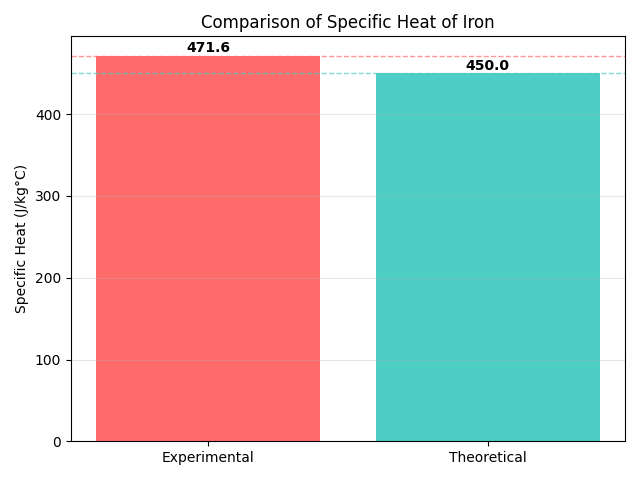
\includegraphics[width=0.8\textwidth]{specific_heat_comparison.png}
    \caption{Comparison of experimental and theoretical specific heat of iron.}
    \label{fig:specific_heat_comparison}
\end{figure}

\section{Error Analysis}
\begin{enumerate}
\item Percentage error for $c_{\text{Fe}}$ compared to literature value (approximately 450 J/kg·K for iron):
\[ \% \text{ error} = \left| \frac{471.6 - 450}{450} \right| \times 100 \approx 4.5\% \]

\item Possible causes of error:
\begin{itemize}
\item Heat loss to surroundings during transfer or experiment (e.g., air currents acting like energy dissipation in wires).
\item Contact between copper container and outer vessel despite efforts to isolate.
\end{itemize}
\end{enumerate}

\section{Results and Discussion}
In this experiment, we determined the specific heat capacity of iron to be $c_{\text{Fe}} = 471.6$ J/kg·K, which is close to the literature value of approximately 450 J/kg·K, with a percentage error of 4.4\%. This validates the conservation of energy principle in heat transfer, as the heat lost by the hot iron was approximately equal to the heat gained by the water and calorimeter, aligning with the zeroth law where the system reaches thermal equilibrium.

However, the slight overestimation suggests systematic errors, primarily heat loss to the environment, which would make the measured $\Delta T$ smaller than ideal, leading to a higher calculated $c_{\text{Fe}}$. Analytically, this highlights the calorimeter's imperfect insulation; a correction factor could be applied by measuring the cooling rate of the system post-equilibrium and extrapolating back using Newton's law of cooling ($dQ/dt = -hA (T - T_{\text{amb}})$) to adjust Q.

Observationally, the small temperature rise (3.1°C) made precise measurement challenging, as minor fluctuations or thermometer resolution limits amplified errors. To address this, we could use a metal with lower specific heat (like lead, $c \approx 130$ J/kg·K) for a larger $\Delta T$, or increase the iron's mass/initial temperature (e.g., to 150°C using an oven) to enhance the signal, potentially reducing relative errors by half. Alternatively, decreasing water volume (while ensuring submersion) could magnify $\Delta T$, though it risks uneven heating---a balance achievable with better stirring techniques.

Why choose iron? Its density ensures it sinks in water for full immersion (unlike less dense materials that might float, complicating heat transfer), and its moderate c allows measurable $\Delta T$ without extremes. Comparing to aluminum ($c \approx 900$ J/kg·K, less dense), $\Delta T$ would be smaller and harder to observe; copper might validate results due to similar properties.

\newpage

\textbf{Student Information}

Name Surname: Hakkı Erdem Günal

Student ID: 173223024

Course: Physics 3 Laboratory

Experiment No / Title: 1 / Determination of Specific Heat of Metals

Experiment Date: October 6, 2025

Submission Date: October 15, 2025

\end{document}